\chapter{Your wish is my command, Reloaded}

\section{Question 1}
This question included adding a feature of choice by our TA. We together determined that this week we would add a multiplayer mode to the game. In Question 2 we will explain the RDD we applied and the UML of the improvements made to the game. 

\section{Question 2}

\subsection{Introduction}

When realising a second player in the game, we came across multiple problems in our structure. The main problem being that it was not a pure Observer Design Pattern. That's where a huge refactoring came in: all elements of Model do not extend SpriteBase anymore but contain one. \\ 
Every instance has a timer of their own and does not require the LevelController to call their update function anymore. (Which was our main problem in our design pattern). \\ \\
Luckily the Player class and its Input class were already set up very well, so that physically adding the second player was easily done. 

\subsection{Multi-Player: Responsibility Driven Design}
We will shortly describe the important classes of the Multi-player feature and how we used Responsibility Driven Design in determining the responsibilities and collaborations of the classes which needed to be changed (or refactored).  

\subsubsection{Observer}
\textit{Responsibility:} \\
The Observer class observes classes which extend the Observable-class. It gets notified by an Observable-object if the object changes and therefor knows when to update in this case the LevelController and/or the ScreenController. \\ \\
\textit{Collaborations:} \\
Both LevelController and ScreenController extend the Observer class and therefore these classes will collaborate. Furthermore the Observer class will also collaborate with the Observable class to be able to get notified when updates are available.

\subsubsection{Observable}
\textit{Responsibility:} \\
The Observable class forms the basis for all classes in the game which easily change state and therefore have to notify for example the ScreenController and the LevelController to determine if for example a level is over. A class which extends the Observable class thus is able to send an update to an Observer class once data in it's class is changed. \\ \\
\textit{Collaborations:} \\
The Observable class forms the basis for all objects in the game and therefore collaborates with Player, Monster, Powerup and Bubble, so that they can send updates. Furthermore an Observable Class can have multiple Observers which it can update. 

\subsubsection{Player}
\textit{Responsibility:} \\
With a multiplayer mode it is of course necessary that there can be multiple Players which can all act autonomous. Therefore each player must have it's own Inputs. \\ \\
\textit{Collaborations:} \\
Player collaborates with Observable to be able to send updates to Observer classes. It collaborates with SpriteBase in order to be able to have x,y coordinate and detect collisions.   

\subsubsection{Monster}
\textit{Responsibility:} \\
With a multiplayer mode a monster has to be able to kill both players. \\ \\
\textit{Collaborations:} \\
Monster collaborates with Observable to be able to send updates to Observer classes. It collaborates with SpriteBase in order to be able to have x,y coordinate and detect collisions. 

\subsubsection{Powerup}
\textit{Responsibility:} \\
Every Powerup should be able to be picked up by both players in multiplayer mode. After being picked up, it should als give the desired Powerup to only the player who picked it up. \\ \\
\textit{Collaborations:} \\
Powerup collaborates with Observable to be able to send updates to Observer classes. It collaborates with SpriteBase in order to be able to have x,y coordinate and detect collisions. 

\subsubsection{Bubble}
\textit{Responsibility:} \\
It must be clear for every bubble who shot the bubble to keep track of who shot a bubble. Points are only given to the player who pops the bubble. \\ \\
\textit{Collaborations:} \\
Bubble collaborates with Observable to be able to send updates to Observer classes. It collaborates with SpriteBase in order to be able to have x,y coordinate and detect collisions. 

\subsubsection{SpriteBase}
\textit{Responsibility:} \\
The Spritebase Class has to owned by all elements in the game after the refactoring. It will still contain all basic information for all elements in the game such as an x,y coordinate and an image. \\ \\
\textit{Collaborations:} \\
Since SpriteBase forms the basis for all elements in the game, it collaborates with Player, Monster, Powerup, Wall and Bubble. 

\newpage
\subsection{Multi-Player: UML}
The UML of the important classes for the Multiplayer and therefore also the refactoring of the game, are displayed in the figure below. 
\begin{center}
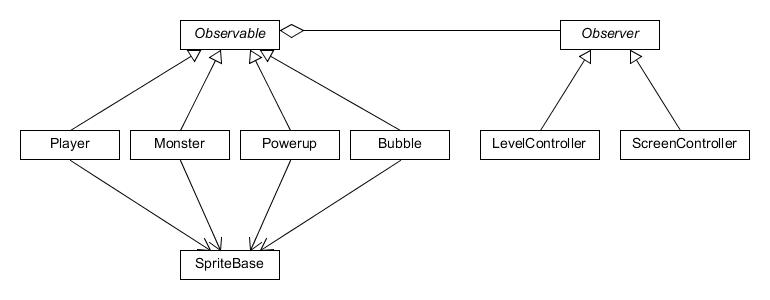
\includegraphics[width=\textwidth]{UML}\\[1cm]	
\end{center}

